% -----------------------------------------------
% chktex-file 44
\documentclass[../index.tex]{subfiles}

% -----------------------------------------------

\begin{document}

% -----------------------------------------------

\renewcommand{\sectiontitle}{Useful WebExtensions APIs and recipes}
\section{\sectiontitle}


% ---------------------------
\renewcommand{\currenttitle}{Permissions}
\begin{frame}[fragile]{\currenttitle}
  Before using any APIs, extensions must \textit{explicitly} specify which APIs
  it wants to use \\[1em]

  We do this in \texttt{manifest.json}:
  \begin{lstlisting}[language=json]
{
  ...
  "permissions": ["*://duckduckgo.com/*", "cookies", "downloads"],
  ...
}
  \end{lstlisting}

  \vspace*{1em}
  The browser can then warn the user at installation time about any potentially
  intrusive behavior.
\end{frame}


% ---------------------------
\renewcommand{\currenttitle}{The \texttt{browser} namespace}
\begin{frame}[fragile]{\currenttitle}
  WebExtensions APIs can be accessed using the \texttt{browser} namespace
  (Firefox + Edge) and \texttt{chrome} namespace (Firefox + Chrome): \\[1em]

  \begin{lstlisting}[language=ES6,basicstyle=\ttfamily\small]
browser.tabs.query({currentWindow: true},
                   console.log)
  \end{lstlisting}

  \vspace*{2em}

  You can also use a \textbf{polyfill} to use \texttt{browser} across all
  browsers:
  \href{https://github.com/mozilla/webextension-polyfill}
       {WebExtension API Polyfill}
\end{frame}

% ---------------------------
\renewcommand{\currenttitle}{Persistent storage}
\begin{frame}[fragile]{\currenttitle}
  The \texttt{storage} API:

  \begin{itemize}
    \item \textbf{can} be used by background scripts
    \item \textbf{cannot} be used by content scripts
    \item \textbf{is async} (\texttt{Promises})
    \item \textbf{requires} the "storage" permission in \texttt{manifest.json}
  \end{itemize}
\end{frame}

% ---------------------------
\begin{frame}[fragile]{\currenttitle}
  Add the "storage" permission to your manifest:
  \begin{lstlisting}[language=json]
...
"permissions": [
  "storage"
],
...
  \end{lstlisting}

  We can now save something to \textit{local} storage in a \textbf{background
  script}:
  \begin{lstlisting}[language=ES6]
browser.storage.local.set()
    .then(() => console.log("Success!"), 
          err => console.log(err));
  \end{lstlisting}
\end{frame}

% ---------------------------
\renewcommand{\currenttitle}{Content script-background script messaging}
\begin{frame}[fragile]{\currenttitle}
  The \texttt{browser.runtime} namespace provides messaging facilities for
  content scripts and background scripts to communicate.

  We can use \textbf{one-off messaging} or \textbf{connection-based messaging}
  (see
  \href{https://developer.mozilla.org/en-US/docs/Mozilla/Add-ons/WebExtensions/Content_scripts#choosing_between_one-off_messages_and_connection-based_messaging}{here}
  to see when you should choose each)
\end{frame}

% ---------------------------
\renewcommand{\currenttitle}{One-off messaging}
\begin{frame}{\currenttitle}
  We can use the following APIs to send and receive one-off messages:

  \begin{table}[h]
    \centering
    \footnotesize
    \begin{tabular}{l |l |l }
              & In content script                     & In background script \\ \hline
      Send    & \texttt{browser.runtime.sendMessage}  & \texttt{browser.tabs.sendMessage} \\
      Receive & \texttt{browser.runtime.onMessage}    & \texttt{browser.runtime.onMessage}
    \end{tabular}
  \end{table}
\end{frame}

% ---------------------------
\renewcommand{\currenttitle}{One-off messaging: example}
\begin{frame}[fragile]{\currenttitle}
  The content script sends a messaage with the URL of a link to the background
  when the user clicks a link: \\[1em]
  \begin{lstlisting}[language=ES6]
// content-script.js
window.addEventListener("click", notifyExtension);

function notifyExtension(e) {
  if (e.target.tagName != "A") {
    return;
  }
  browser.runtime.sendMessage({"url": e.target.href});
}
  \end{lstlisting}
\end{frame}

% ---------------------------
\begin{frame}[fragile]{\currenttitle}
  The background script listens and displays a notification with the URL: \\[1em]

  \begin{lstlisting}[language=ES6]
// background-script.js
browser.runtime.onMessage.addListener(notify);

function notify(message) {
  browser.notifications.create({
    "type": "basic",
    "iconUrl": browser.extension.getURL("link.png"),
    "title": "You clicked a link!",
    "message": message.url
  });
}
  \end{lstlisting}
\end{frame}

% ---------------------------
\renewcommand{\currenttitle}{Connection-based messaging}
\begin{frame}[fragile]{\currenttitle}
  A connection is useful for sending many messages back-and-forth. \\

  \begin{enumerate}
    \item One side listens for connections using \texttt{runtime.onConnect}
    \item The other side tries to make a connection
      \begin{itemize}
        \item \texttt{tabs.connect()} if inside a background script
        \item \texttt{runtime.connect()} if inside a content script
      \end{itemize}
  \end{enumerate}
  In this example, the background script:

  \begin{itemize}
    \item Listens for connection attempts
    \item Stores the port (to send returning messages on later)
    \item Listens for messages received and logs them
    \item Sends messages to content script periodically
  \end{itemize}

\end{frame}

% ---------------------------
\renewcommand{\currenttitle}{Connection-based messaging: example}
\begin{frame}[fragile]{\currenttitle}
  The content script:
  
  \begin{itemize}
    \item Connects to the background script
    \item Stores the port (to send and receive messages on)
    \item Listens for messages received and logs them
    \item Sends messages to background script on click
  \end{itemize}
\end{frame}

% ---------------------------
\renewcommand{\currenttitle}{Connection-based messaging: example}
\begin{frame}[fragile]{\currenttitle}
  \begin{lstlisting}[language=ES6]
// background-script.js
let portFromCS;

browser.runtime.onConnect.addListener(p => {
  portFromCS = p;
  portFromCS.postMessage({greeting: "hi there content script!"});
  portFromCS.onMessage.addListener(function(m) {
    portFromCS.postMessage({
      greeting: "In bg, received message from cs:" + m.greeting
    });
  });
});

setInterval(() => {
  portFromCS.postMessage({greeting: "periodic message!"})
}, 3000)
  \end{lstlisting}
\end{frame}

% ---------------------------
\begin{frame}[fragile]{\currenttitle}
  \begin{lstlisting}[language=ES6]
// content-script.js
let myPort = browser.runtime.connect({name: "port-from-cs"});
myPort.postMessage({greeting: "hello from content script"});

myPort.onMessage.addListener(function(m) {
  console.log("In cs, received message from bg:");
  console.log(m.greeting);
});

document.body.addEventListener("click", function() {
  myPort.postMessage({greeting: "they clicked the page!"});
});
  \end{lstlisting}
\end{frame}

% ---------------------------
\renewcommand{\currenttitle}{Modifying context menus}
\begin{frame}[fragile]{\currenttitle}
  We can add items to the right-click context menu with the \texttt{menus} API.
  \\[1em]

  This requires the "menus" permission:
  \begin{lstlisting}[language=json]
{
  ...
  "permissions": [..., "menus"],
  ...
}
  \end{lstlisting}
\end{frame}

% ---------------------------
\renewcommand{\currenttitle}{Modifying context menus: example}
\begin{frame}[fragile]{\currenttitle}
  An example of what can be done: \\[2em]

  \begin{center}
    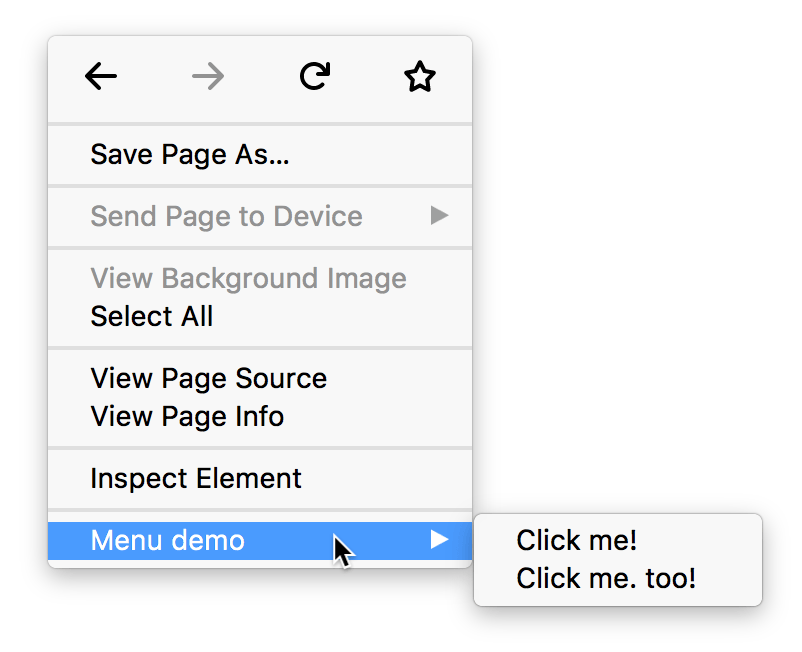
\includegraphics[width=0.6\textwidth]{\subdir/02-apis-menus.png}
  \end{center}
\end{frame}

% ---------------------------
\begin{frame}[fragile]{\currenttitle}
  We use the \texttt{menus} (Firefox) or \texttt{contextMenus} (Firefox,
  Chrome, Edge, Opera) namespaces from \textbf{background scripts}: \\[1em]

  Specifically, \texttt{browser.menus.create} adds a menu item.
\end{frame}

% ---------------------------
\begin{frame}[fragile]{\currenttitle}
  \begin{lstlisting}[language=ES6]
function onCreated() {
  if (browser.runtime.lastError) {
    console.log("Error: " + browser.runtime.lastError);
  } else {
    console.log("Item created successfully");
  }
}

browser.menus.create({
  id: "click-me",
  title: "Click me!",
  contexts: ["all"]
}, onCreated);
  \end{lstlisting}
\end{frame}

% ---------------------------
\begin{frame}[fragile]{\currenttitle}
  We can use \texttt{browser.menus.onClicked} to perform appropriate actions
  when the menu item has been clicked: \\[1em]
  \begin{lstlisting}[language=ES6]
browser.menus.onClicked.addListener((info, tab) => {
  switch (info.menuItemId) {
    case "click-me":
      console.log("Click me! clicked!");
      break;
  }
});
  \end{lstlisting}
\end{frame}

% -----------------------------------------------

\end{document}
